\section{Auswertung}

Alle Ausgleichsrechnungen werden mit dem Paket \texttt{scipy.optimize.curve\_fit}  aus \texttt{Python 3.7.3} durchgeführt.
Für Rechnungen mit fehlerbehafteten Größen wird das Paket \texttt{uncertainties} aus \texttt{Python 3.7.3} verwendet.\\

\subsection{Justage}
Zunächst wird eine Temperaturmessung und Justage durchgeführt. Mithilfe eines digitalen Thermometers wird die Temperatur
auf \SI{21.5}{\degreeCelsius} bestimmt. Nach dem Einstellen der in der Versuchsanleitung \cite{anleitung} aufgeführten Startwerte
werden diese solange variiert bis die gewünschten Signale zu sehen sind.
Die richtige Frequenz ist daran zu erkennen, dass das gemessene Signal keine Schwingungen mehr aufweist. Ist die richtige Frequenz
eingestellt wird die Phase variiert ist es das Ziel, dass sich das gesamte Signal ausschließlich im Realteil befindet.
Das bedeutet es wird versucht die Phase so zu verändern, dass eines der beiden angezeigten Signale möglichst verschwindet.
Beim Einstellen der Gradienten ist darauf zu achten, dass das FID-Signal möglichst lange zu erkennen ist.
Unter Berücksichtigung dieser Vorgehensweisen ergeben sich
\begin{align*}
  \text{Frequenz}&=\SI{21.72088}{\mega\hertz} \\
  \text{Phase} &= \SI{30}{\degree} \\
    x&=–1,7 \\
    y&=–5,1 \\
    z&=3,7 \\
    z^2 &=–2,4
\end{align*} \noindent
für die eingestellten Werte. \\
Die Bestimmung der Pulslängen für den $\SI{90}{\degree}$- und $\SI{180}{\degree}$-Puls ergibt
\begin{align*}
  \SI{180}{\degree} &= \SI{5.04}{\micro\second}\\
  \SI{90}{\degree}  &= \SI{2.52}{\micro\second}.
\end{align*} \noindent

\subsection{$T_1$-Messung}
Zur Bestimmung der $T_1$-Zeit wird die Magnetisierung für verschiedene Pulsabstände $\tau$ bestimmt.
Eine solche Messung ist beispielhaft in Abbildung \ref{fig:t1} dargestellt. Deutlich wird, dass eine vollständige Unterdrückung
des Imaginärteils, dargestellt durch den grünen Graphen, nicht gelungen ist. Außerdem sind zwei Ausschläge zu erkennen, wobei der
erste dem $\SI{180}{\degree}$-Puls zuzuordnen ist und der zweite dem $\SI{90}{\degree}$-Puls, der in diesem
Versuchsteil untersucht werden soll.
\begin{figure}[H]
  \centering
  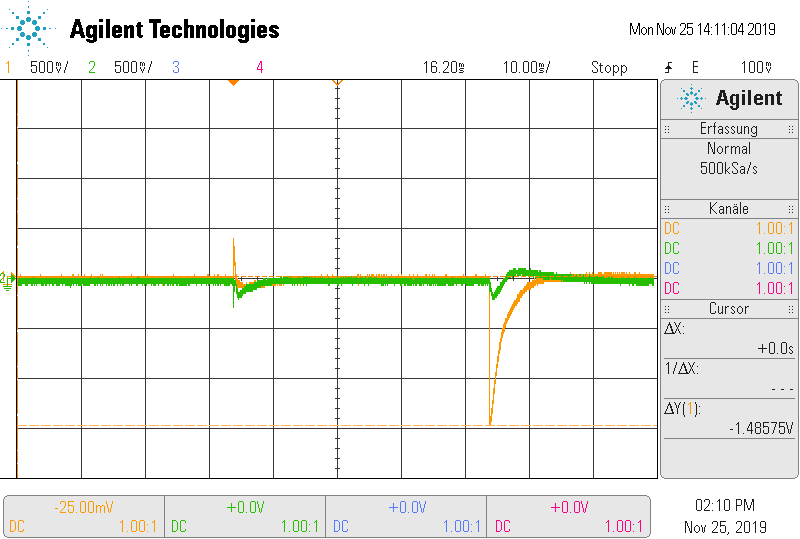
\includegraphics[width=0.8\textwidth]{../data/T1.png}
  \caption{Beispielhafte Darstellung einer Messung zur Bestimmung der $T_1$-Relaxationszeit. Untersucht wird der zweite zu
  erkennende Ausschlag, da er dem $\SI{90}{\degree}$-Puls zugeordnet ist. Beachtet wird dabei nur der Realteil des Signals,
  der durch den \textcolor{orange}{orangen} Graphen repräsentiert wird.}
  \label{fig:t1}
\end{figure} \noindent
Die bei der Messung mithilfe der Cursorfunktion bestimmten Signalstärken sind in Abbildung \ref{fig:t1_fit} gegen den
jeweiligen Pulsabstand $\tau$ zusammen mit einer Ausgleichskurve aufgetragen.
\begin{figure}[H]
  \centering
  \includegraphics[width=0.9\textwidth]{../Auswertung/t1_fit.pdf}
  \caption{Die aufgenommen Messwerte der Signalstärke in Abhängigkeit der Pulslänge $\tau$, sowie die
  zur Bestimmung der $T_1$-Zeit durchgeführte Ausgleichskurve. Für die x-Achse wird eine
  logarithmische Achse verwendet.}
  \label{fig:t1_fit}
\end{figure}
Durch die aufgenommenen Messwerte wird ein Ausgleichgraph der Form
\begin{equation*}
  M(\tau) = M_0 \cdot \exp(–\tau/T_1) + M_1
\end{equation*}
gelegt. Diese Regression liefert
\begin{align*}
  T_1 &= \SI{1.35(005)}{\second} \\
  M_0 &= \SI{3.00(005)}{\volt} \\
  M_1 &= \SI{-1.40(005)}{\volt}
\end{align*} \noindent
für die Relaxationszeit $T_1$, sowie die Magnetisierungsparameter $M_0$ und $M_1$.
Idealerweise stehen die Parameter $M_0$ und $M_1$ im Zusammenhang mit $M_0 = -2M_1$ \cite{anleitung}. Bei den durch die Regession bestimmten
Werten ergibt sich ein Verhätnis von
\begin{equation*}
  \frac{M_0}{M_1} = 2.22.
\end{equation*}
Das bedeutet, dass durch die durchgeführte Justage nicht die exakten Einstellungen vorgenommen worden sind. Dies lässt
sich zum Einen auch schon daran erkennen, dass sowohl Real- als auch Imaginärteil noch zu erkennen sind.

\subsection{$T_2$-Messung}
Im ersten Versuchsteil zur Bestimmung der $T_2$-Zeit wird der MG-Schalter auf \textit{on} gestellt. Somit
wird hier die Meiboom-Gill-Methode angewendet.
In Abbildung \ref{fig:t2} ist das aufgenommene Signal dargestellt. Es ist gut zu erkennen, das es den gewünschten Verlauf mit vielen Echosignalen zeigt.
\begin{figure}[H]
  \centering
  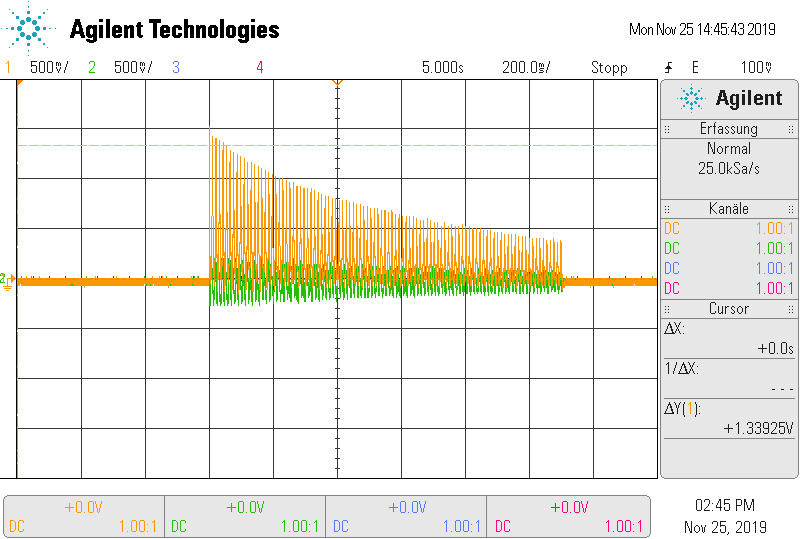
\includegraphics[width=0.8\textwidth]{../data/T2.png}
  \caption{Das aufgenommene Signal zeigt bei der Meiboom-Gill-Methode den gewünschten Verlauf. Die Signalstärke ist nach dem
  100. Maximum auf ca. $\frac{1}{3}$ der Maximalhöhe abgefallen. In \textcolor{orange}{orange} ist der untersuchte
  Realteil des Signals zu sehen.}
  \label{fig:t2}
\end{figure} \noindent
Zur Bestimmung der Relaxationszeit $T_2$, wird eine Ausgleichskurve der Form
\begin{equation*}
  M(t) = M_0 \cdot \exp(–t/T_2) + M_1
\end{equation*}
an die Einhüllende des oszilliereden Signals angepasst.
Dazu werdend die Maxima der Werte bestimmt und diese zur Berechnung des Ausgleichsgraphen verwendet.
Diese ist zusammen mit den Messwerten in Abbildung \ref{fig:T2_fit}
dargestellt.
\begin{figure}[H]
  \centering
  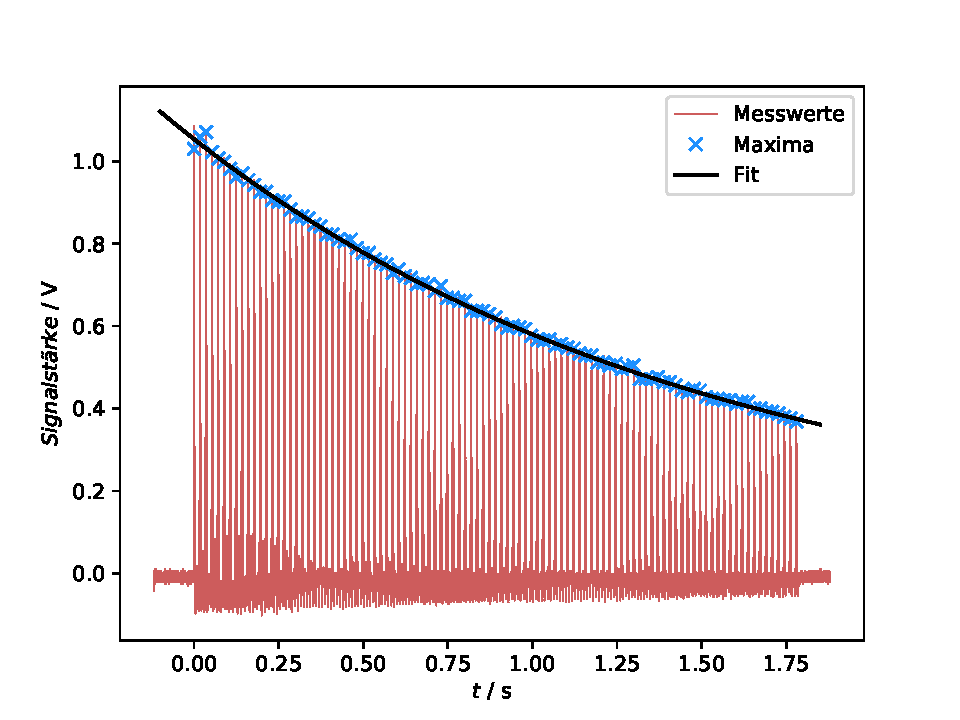
\includegraphics[width=0.9\textwidth]{../Auswertung/T2_fit.pdf}
  \caption{Die zur Bestimmung der $T_2$-Zeit durchgeführte Ausgleichsrechnung. In \textcolor{indianred}{rot} ist die Ausgleichskurve zu erkennen,
  die an die Einhüllende (\textcolor{dodgerblue}{blau}) des oszillierenden Signals (\textcolor{gray}{grau}) angepasst wird.}
  \label{fig:T2_fit}
\end{figure} \noindent
Die Regression liefert
\begin{align*}
  %M_0 &=  \SI{4791977.76(352863663)}{\milli\volt} \\
  %M_1 &=  \SI{188.18(5080)}{\milli\volt} \\
  T_2 &=  \SI{0.56(005)}{\second}
\end{align*}
für die gesuchte Spin-Spin-Realaxationszeit $T_2$. \\
Im Vergleich dazu ist in Abbidung \ref{fig:t2_off} das aufgenommene Signal für die Carr-Purcell-Methode zu sehen. Das heißt bei diesem
Messteil ist der MG-Schalter auf \textit{off} gestellt.
\begin{figure}[H]
  \centering
  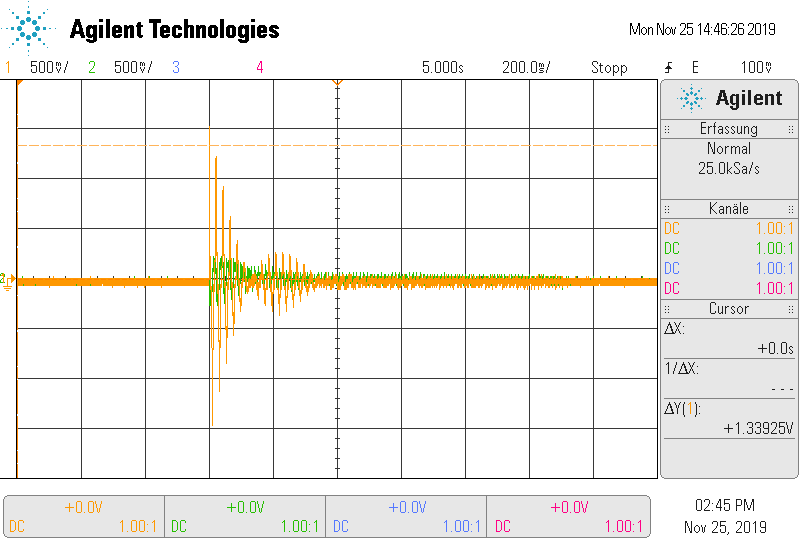
\includegraphics[width=0.8\textwidth]{../data/scope_76.png}
  \caption{Das aufgenommene Signal für die Carr-Purcell-Methode. Dabei ist deutlich zu erkennen, dass es durch die angelegten
  $\SI{180}{\degree}$-Pulse zum Wechsel zwischen Maxima im positiven und negativen Bereich kommt. Zusätzlich kommt es durch einen nicht exakt eingestellten \SI{180}{\degree}-Puls zu einer Schwebung, da die Magnetisierung nie genau auf die x-y-Ebene gekippt wird und so das Signal stärker abnimmt um scich dann wieder aufzubauen. Dabei repräsentiert der \textcolor{orange}{orangene} Verlauf den Realteil des Signals und der \textcolor{green}{grüne} Veraluf den Imaginärteil.}
  \label{fig:t2_off}
\end{figure} \noindent
Es wird deutlich, dass im Gegensatz zu dem aufgenommenen Signal der Meiboom-Gill-Methode bei dieser Aufnahme die Maxima zwischen
dem positiven und negativen Bereich alternieren. Dies ist auf die geschalteten $\SI{180}{\degree}$-Pulse zurückzuführen.
Weiterhin nimmt das Signal deutlich schneller ab, als mit der Meiboom-Gill-Methode, weiterhin ist eine Schwebung in dem Signal zu erkennen. Dies ist auf die Ungenauigkeit der geschalteten \SI{180}{\degree}-Pulse zurückzuführen.
Zur Verdeutlichung des typischen Verlaufs eines Spin-Echo Signals ist in Abbildung \ref{fig:N1} ein Signal dargestellt mit nur einem
geschalteten B-Puls.
\begin{figure}[H]
  \centering
  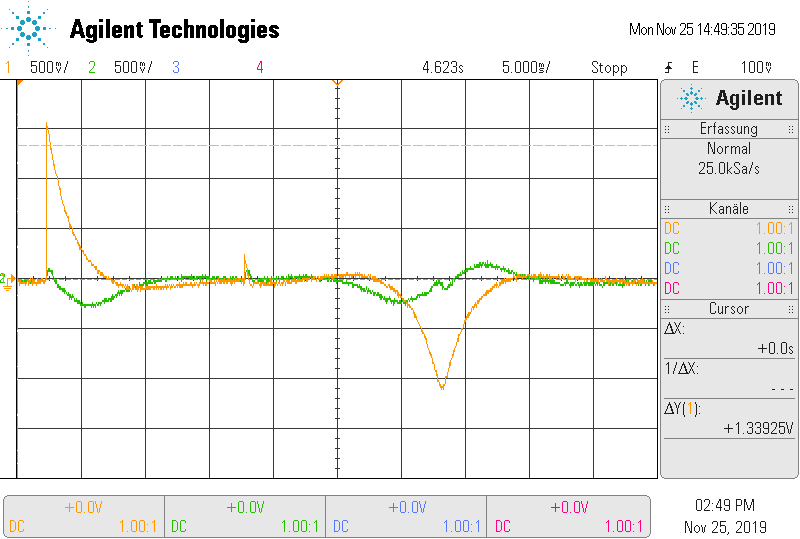
\includegraphics[width=0.8\textwidth]{../data/scope_77.png}
  \caption{Das aufgenommene Signal, wenn nur ein einziger B-Puls geschaltet ist. Zu Beginn des Signals ist der
  $\SI{90}{\degree}$-Puls zu erkennen. Nach dem $\SI{180}{\degree}$-Puls baut sich das Signal durch die Rephasierung
  wieder auf. Dabei repräsentiert der \textcolor{orange}{orangene}
  Verlauf den Realteil des Signals und der \textcolor{green}{grüne} Veraluf den Imaginärteil.}
  \label{fig:N1}
\end{figure} \noindent
Zu erkennen ist zu Beginn des aufgenommenen Signals der $\SI{90}{\degree}$-Puls, der die Magnetisierung in die x-y-Ebene kippt.
Daraufhin kommt es zur Dephasierung der Spins mit der $T_2$-Zeit. Der $\SI{180}{\degree}$-Puls, der durch einen kleinen Ausschlag
zwischen dem Maximum und Minimum zu erkennen ist, sorgt für eine Rephasierung. Diese führt zu einem messbaren Signal, welches
jedoch aufgrund der Spin-Gitter-Wechselwirkung eine geringere Signalstärke aufweist.

\subsection{Diffusionsmessung}
In Abbildung \ref{fig:diff_fit} sind die gemessenen Echohöhen gegen den Pulsabstand $\tau$ auftragen.
Zusätzlich dazu wird eine Ausgleichskurve der Form
\begin{equation*}
  M(\tau) = M_0 \cdot \exp(–2\tau/T_2)\cdot \exp(–\tau^3/T_D) + M_1
\end{equation*}
mithilfe der Messwerte bestimmt. Dabei beschreibt $T_D$ die Diffusionszeit. Zur Bestimmung der gesuchten Parameter wird
die zuvor bestimmte $T_2$-Zeit verwendet.
\begin{figure}[H]
  \centering
  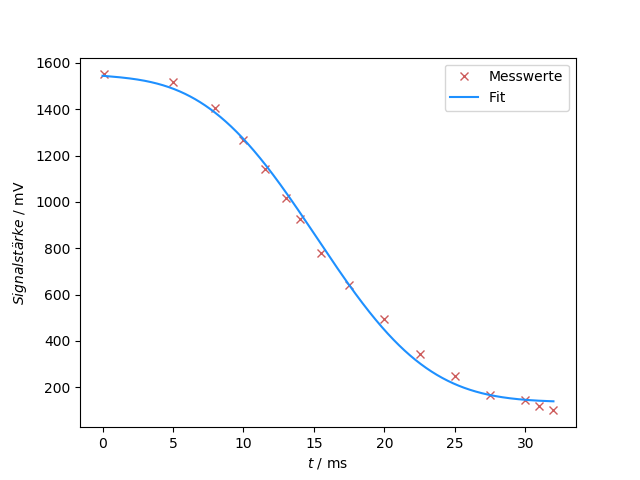
\includegraphics[width=0.8\textwidth]{../Auswertung/Diff_fit.png}
  \caption{Die gemessenen Echohöhen aufgetragen gegen den Pulsabstand $\tau$. Zur Bestimmung der Diffusionszeit $T_D$ wird eine
  Ausgleichskurve bestimmt.}
  \label{fig:diff_fit}
\end{figure} \noindent
Die Regression liefert
\begin{align*}
  M_0 &= \SI{1.41(002)}{\volt} \\
  M_1 &= \SI{0.14(002)}{\volt} \\
  T_D &= \SI{5.57(025)e-6}{\second}
\end{align*}
für die gesuchten Parameter.
Mithilfe des Zusammenhangs in Gleichung \eqref{eqn:TDiffusion}
kann die Diffusionskonstante bestimmt werden. Dabei beschreibt G den Gradienten des Magnetfelds $B_0$ , der mittels Fouriertransformation eines Echos
bestimmt wird. In Abbildung \ref{fig:echo_vorher} ist das verwendete Echo bei einem Pulsabstand von $\tau = \SI{0.0155}{\second}$ dargestellt. Wobei sowohl der Imaginär- als auch der Realteil
zu sehen sind.
\begin{figure}[H]
  \centering
  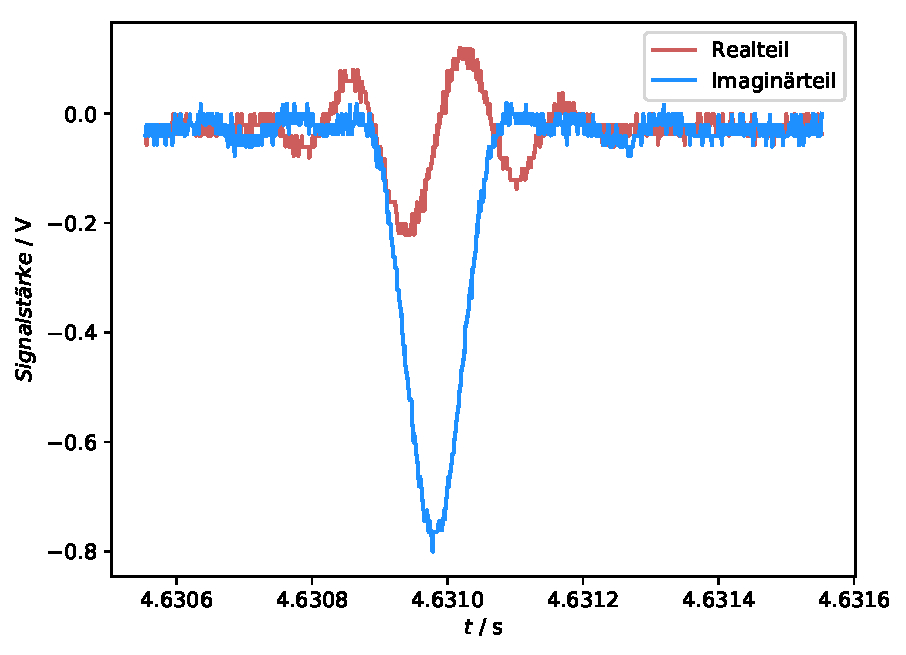
\includegraphics[width=0.9\textwidth]{../Auswertung/echo_vorher.pdf}
  \caption{Das zur Berechnung des Gradienten verwendete Echo bei einem Pulsabstand von $\tau = \SI{0.0155}{\second}$
  vor dem Abschneiden am Maximum und der durchgeführten
  Phasenkorrektur. In \textcolor{indianred}{rot} ist der Real- und in \textcolor{dodgerblue}{blau} der Imaginärteil des Signals dargestellt.}
  \label{fig:echo_vorher}
\end{figure} \noindent
Bevor eine Fouriertransformation durchgeführt werden kann, müssen die Messwerte des Signals so dargestellt werden, dass sie
beim Maximum des Realteils des Signals starten. Diese veränderte Darstellung des Signals ist zur Verdeutlichung des Vorgehens in
Abbildung \ref{fig:echo_ab} visualisiert.
\begin{figure}[H]
  \centering
  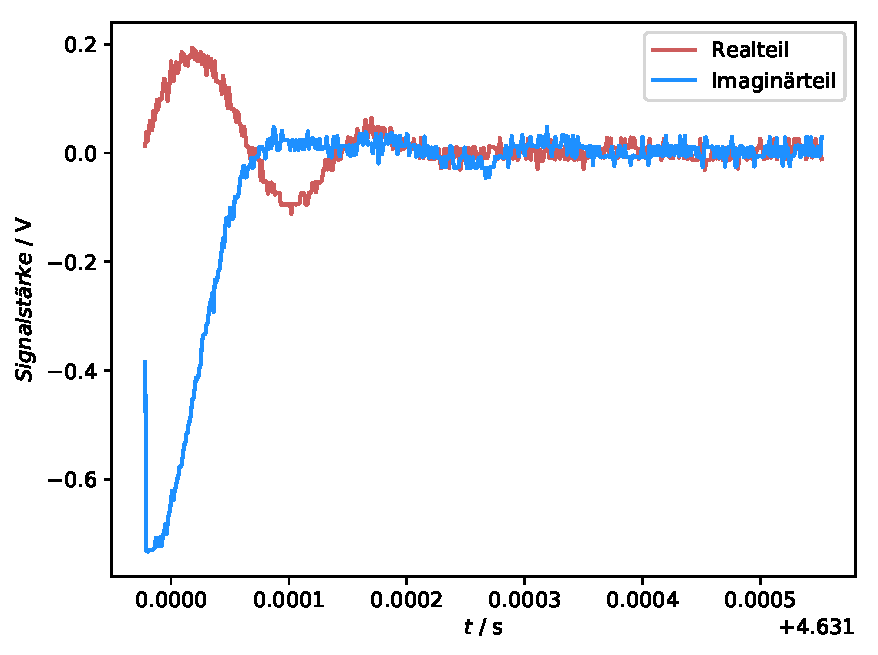
\includegraphics[width=0.9\textwidth]{../Auswertung/echo_phasenkorrektur.pdf}
  \caption{Das zur Fouriertransformation vorbereitete Signal nach der Phasenkorrektur. Zu sehen sind sowohl der Realteil (\textcolor{indianred}{rot}) als auch der
  Imagainärteil (\textcolor{dodgerblue}{blau}) des Signals, beginnend beim Maximum des gemessenen Imaginärteils.}
  \label{fig:echo_ab}
\end{figure} \noindent
In Abbildung \ref{fig:ft} ist das zu Abbildung \ref{fig:echo_ab} gehörige Frequenzspektrum abgebildet, das mithilfe der
Fouriertransformation bestimmt wird. Dieses Spektrum gibt die Verteilung der Larmorfrequenzen der Protonen wieder.
Aufgrund des geschalteten Gradienten unterscheidet diese sich abhängig vom Ort der Protonen.
\begin{figure}[H]
  \centering
  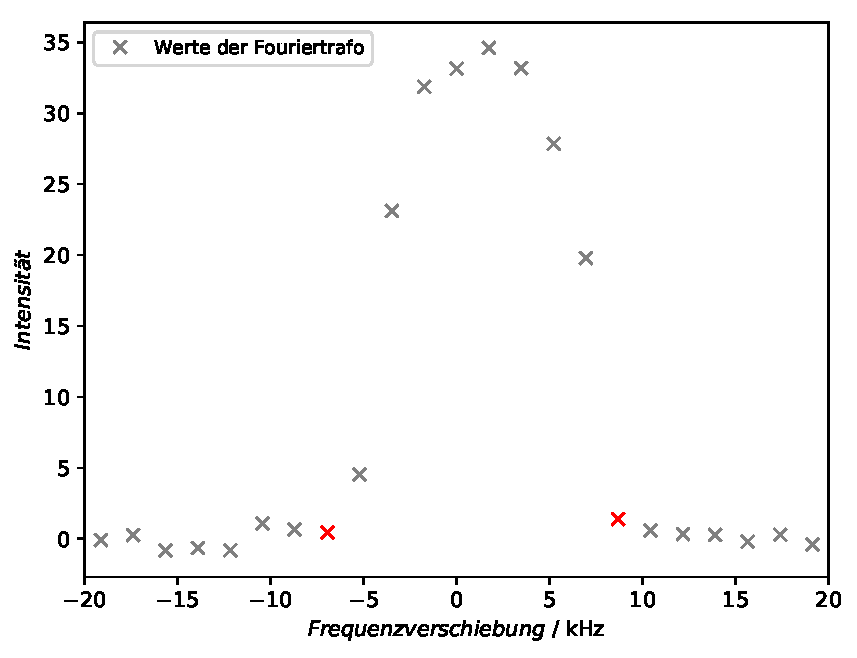
\includegraphics[width=0.9\textwidth]{../Auswertung/echo_ft.pdf}
  \caption{Das Ergebnis der auf das Echo angewendete Fouriertransformation. Mithilfe der Bestimmung der Breite der Frequenzverbreiterung
  ist es möglich den Gradienten und darüber die Diffusionskonstante zu berechnen.}
  \label{fig:ft}
\end{figure} \noindent
Die Frequenzbreite wird zwischen den beiden rot dargestellten Messwerten zu
\begin{align*}
  d_f = \SI{15.65}{\kilo\hertz}
\end{align*}
bestimmt.
Damit ist es über den Zusammenhang
\begin{align*}
  G = \frac{2\pi d_f}{\gamma d}
\end{align*}
möglich den vorliegenden Gradienten zu
\begin{align}
  G = \SI{0.088}{\tesla\per\meter}
\end{align}
zu bestimmen. Dabei wird mit $d = \SI{4.2}{\milli\meter}$ der Durchmesser des Probenröhrchens verwendet.
Mit dem bestimmten Grradienten und Gleichung \eqref{eqn:TDiffusion} kann die Diffusionskonstante zu
\begin{align}
  D = \SI{2.88(26)e-10}{\square\meter\per\second}
\end{align}
bestimmt werden.
Daraus ergibt sich mit einer Viskosität von $\eta \approx \SI{2.95}{\milli\pascal\second}$ \cite{viso} und einer
Temperatur von ca. $\SI{21.5}{\degreeCelsius}$
mithilfe von Formel \eqref{eqn:stokes}
\begin{align}
  r = \SI{2.54(22)}{\angstrom}
  \label{eqn:radius1}
\end{align}
für den Molekülradius des verwendeteten 1-Butanol. \\
Zum Vergleich wird der Molekülradius mithilfe des Molekulargewichtes und der Dichte berechnet. Dabei wird die Annahme getroffen,
dass die Moleküle in der vorliegenden Flüssigkeit eine hexagonal dichteste Kugelpackung bilden.
Da die Packungsdichte einer hexagonal dichtesten Kugelpackung mit
\begin{align*}
  \frac{\pi}{3\sqrt{2}} \approx \SI{74}{\percent}
\end{align*}
bekannt ist, ergibt sich für die Dichte
\begin{align*}
  \rho &= \frac{m_\text{ges}}{V_\text{ges}} \\
       &= \frac{\pi m_\text{But}}{3\sqrt{2}V_\text{But}}\,.
\end{align*}
Unter der Annahme, dass die 1-Butanol-Moleküle kugelförmig sind und somit für ihr Volumen
\begin{align*}
  V_\text{But} = \frac{4}{3} \pi r^3
\end{align*}
gilt, ergibt sich für den gesuchten Molekülradius
\begin{align}
  r = \sqrt[3]{\frac{m_\text{But}}{4\sqrt{2}\rho}} \approx \SI{2.99}{\angstrom}\, .
  \label{eqn:radius2}
\end{align}
Dabei wird $m_\text{But}$ mithilfe einer Molaren Masse von $\SI{74.12}{\gram\per\mole}$ berechnet.
Die Dichte von 1-Butanol beträgt bei Raumtemperatur ca. $\SI{0.81}{\gram\per\cubic\meter}$ \cite{dichte}.
